%
% File main.tex
%
% NLP course project-proposal template, Warsaw University of Technology.
% Prepared by Anna Wróblewska, adapted from the ACL 2015 conference
% formatting template (acl2015.sty), originally by the ACL 2015
% organizers and earlier ACL/EACL format authors (see acl2015.pdf
% for the full credits chain).

\documentclass[11pt]{article}
\usepackage{acl2015}
\usepackage[T1]{fontenc}
\usepackage{times}
\usepackage{url}
\usepackage{latexsym}
\usepackage{xcolor}
\usepackage{longtable}
\usepackage{graphicx}
\usepackage{booktabs}
\usepackage{float}

\renewcommand{\dbltopfraction}{0.95}
\renewcommand{\dblfloatpagefraction}{0.5}
\setcounter{dbltopnumber}{2}
\raggedbottom

\setlength\titlebox{8.5cm} 

\title{Phase 1: Project Proposal\\Four press regimes, one century: Polish headlines from the interwar market to the feed}

\author{Gabriela Majstrak \\
  327204 \\
  {\tt 01180624@pw.edu.pl} \\\And
  Jan Opala \\
  329823 \\
  {\tt 01180728@pw.edu.pl} \\ \AND
  Anna Ostrowska \\
  327300 \\
  {\tt 01180729@pw.edu.pl} \\\And
  Zofia Sasimowska \\
  313530 \\
  {\tt 01161618@pw.edu.pl} \\ \AND
  supervisor: Soveatin Kuntur\\
  Warsaw University of Technology \\
  {\tt soveatin.kuntur.dokt@pw.edu.pl}}

\date{}

\begin{document}
\maketitle

{\small\em Template: Anna Wróblewska (Warsaw University of Technology), adapted from the ACL 2015 conference formatting template.}
\vspace{4pt}

\begin{abstract}
Clickbait is usually attributed to the online attention economy. Polish press allows a test: within one century it passed through four regimes, from the interwar market through occupation and communist censorship to a restored market. We ask whether attention-capturing methods in front-page headlines are more frequent under market conditions. Our review of large language model (LLM) annotation, scan-to-text pipelines, clickbait detection and Polish press corpora finds no corpus of occupation press and no annotated Polish clickbait benchmark. We propose a corpus of about 7,000 headlines, per-period measurement of optical character recognition (OCR) quality, a regime comparison with bootstrap confidence intervals, and a temporal-transfer test of classifiers.
\end{abstract}

\section{Introduction}
Clickbait is usually explained by the online attention economy, yet newspapers competed for readers long before the internet, and large-scale studies of headline style focus on recent online news \cite{nickl2025evolution,blom2015clickbait}. Polish press allows a test: within one century it passed through a free market (1918--1939), German occupation (1939--1945), censorship in the Polish People's Republic (PRL, 1945--1989) and a restored market (1989--now). If attention-capturing methods follow competition, they should be more frequent in the two market periods.

\paragraph{Research questions and hypotheses.}
\textbf{RQ1:} Are devices such as forward-reference, curiosity gaps or emotional wording more frequent in market-period front-page headlines? (H1: yes.)
\textbf{RQ2:} How accurately can headlines be recovered from scans in each period, and does the error bias RQ1? (H2: OCR error differs by period.)
\textbf{RQ3:} Do classifiers trained on contemporary headlines detect devices in older periods? (H3: performance drops with temporal distance.)

\paragraph{Research gaps.}
No corpus covers the occupation press or compares headlines across regimes (G1) \cite{Pawłowski_2024,ogrodniczuk-etal-2026-polish}; Polish press collections report no per-period OCR error (G2) \cite{kaye2026petroleum}; there is no annotated Polish clickbait benchmark (G3); clickbait classifiers have not been tested on much older texts, and LLM annotators have not been evaluated on Polish historical headlines (G4) \cite{andelic2025clic,dobranić2026approachesanalysinghistoricalnewspapers}.

\paragraph{Expected deliverables.}
(1) About 7,000 labeled front-page headlines from four periods (post-1939 as text only); (2) a pipeline report with headline-detection precision/recall and character error rate per period; (3) a regime comparison with confidence intervals and a temporal-transfer test.

\section{State of the Art}
Table~\ref{tab:sota} lists each reviewed work with its data and results; below we discuss the gaps each area leaves.

\begin{table*}[!tp]
\centering
\scriptsize
\setlength{\tabcolsep}{3pt}
\begin{tabular}{@{}p{3.5cm} p{4.4cm} p{3.7cm} p{3.75cm}@{}}
\toprule
\textbf{Work} & \textbf{What it does} & \textbf{Dataset (split)} & \textbf{Result} \\ \midrule
\newcite{bavaresco2025llmsinsteadhumanjudges}: \emph{LLMs instead of Human Judges? A Large Scale Empirical Study across 20 NLP Evaluation Tasks} & Tests whether 11 LLMs can replace human judges; introduces JUDGE-BENCH (20 human-annotated datasets) & 20 mostly English datasets, test only ($>$70k items), e.g.\ CoLA, ToxicChat, DICES, SummEval, NewsRoom, WMT 2020/2023, ROSCOE & Agreement low and uneven across tasks (GPT-4o: mean Cohen's $\kappa$ = 0.28 categorical, Spearman's $\rho$ = 0.50 graded; Llama-3.1-70B ties on $\kappa$) \\
\newcite{Kucia_2026}: \emph{LLM Essay Scoring Under Holistic and Analytic Rubrics: Prompt Effects and Bias} & Compares open-weight LLM and human essay scores, holistic (one grade) and analytic (traits such as grammar), under two prompt styles & ASAP 2.0 (24,728 essays), ELLIPSE (6,482), DREsS (8,487); zero-shot, no fine-tuning (original train and test sets both scored) & Holistic grades fairly close (best Llama-3.1-70B, quadratic weighted kappa 0.60 on ASAP 2.0); trait scores much harsher, esp.\ grammar and conventions ($\approx$1 point lower on a 5-point scale) \\
\newcite{Gilardi_2023}: \emph{ChatGPT outperforms crowd workers for text-annotation tasks} & Compares zero-shot ChatGPT with Amazon Mechanical Turk (MTurk) workers on annotating tweets and news articles (relevance, stance, topics, frames) & 4 datasets, 6,183 tweets and news articles (2017--2023); trained annotators as gold; evaluation only (no training split) & About 25 percentage points more accurate than MTurk on average; relevance accuracy 59--83\%; about 30$\times$ cheaper per annotation \\
\newcite{dobranić2026approachesanalysinghistoricalnewspapers}: \emph{Approaches to Analysing Historical Newspapers Using LLMs} & Compares four LLMs on sentiment towards social groups in OCR-degraded historical Slovene newspapers & sPeriodika (\emph{Slovenec}, \emph{Slovenski narod}); 371 hand-labelled mentions from three newspapers (test only) & Best accuracy 0.695 (GaMS3-12B); neutral reliable (F1 0.79), negative over-assigned, positive often missed (recall 0.30) \\
\midrule
\newcite{Pawłowski_2024}: \emph{Korpus prasy polskiej ChronoPress jako infrastruktura i narzędzie badań medioznawczych} [ChronoPress Polish press corpus as infrastructure and a tool of media studies] & Describes ChronoPress, a sampled corpus of the PRL press, and tracks words over time with lexical time series & 1945--1966; $\sim$6,000 samples of $\sim$300 words per year ($\sim$40M tokens), chosen by readership segment; article title in XML metadata; no train/test split & Resource paper, no metric. E.g.\ ``Katowice'' nearly disappears in 1953--1956, when the city was called Stalinogród \\
\newcite{ogrodniczuk-etal-2026-polish}: \emph{The Polish PressMint Corpus} & Polish part of CLARIN PressMint: three press subcorpora in TEI XML (Text Encoding Initiative), annotated with Hydra (lemmas, Universal Dependencies tags and parses, named entities) & Short Press (206k words) and Journalistic (204k), both 1830--1918; InterWar 6.5M words (1918--1939, 6 periodicals); no train/test split & Resource paper, no metric; InterWar has manually marked article titles \\
\newcite{kaye2026petroleum}: \emph{Petroleum and Press --- Concepts about Oil in Polish Periodical Press, 1853--1918} & Harvests periodicals mentioning petroleum from Polona via its API, re-segments them (Eynollah) and re-OCRs them (Tesseract, OCR-D workflow) & 18,361 issues of $\sim$800 non-daily periodicals (1853--1918) selected by keyword; $\sim$470 GB; CC0; no train/test split & Resource paper, no CER: OCR only spot-checked by hand and judged ``excellent''; layout detection about 4 minutes per page \\
\newcite{kie:etal:26}: \emph{The Corpus of Contemporary Polish --- a New Reference Corpus with Rich Syntactic Annotations} & KWJP reference corpus with automatic Hydra annotation (lemmas, tags, named entities, syntax trees) & 2011--2020; $\sim$100M balanced (45\% press) + $\sim$1.4B unbalanced tokens; no internet texts. Tested on held-out NKJP1M (National Corpus of Polish subset) and 10\% of treebanks & NKJP1M: tags F1 97.99\%, lemmas F1 98.48\%; treebank test: unlabelled / labelled attachment 96.29\% / 91.04\% \\
\midrule
\newcite{koynov2025opportunities}: \emph{Opportunities and Challenges of LLMs as Post-OCR Correctors} & Prompts LLMs (Llama 3.3 70B, GPT-4o mini and its fine-tuned version) to correct OCR output without access to the scans & BLN600 (600 pages of English newspaper crime reports, 1834--1894), OCR-D-GT (217 German pages), ICDAR2019 (English and German library material) & Character error rate (CER) drops on cleaner text (GPT-4o mini, BLN600: 0.072 to 0.031); on noisy OCR-D-GT LLMs hallucinate and CER rises 19\% (GPT-4o mini) and 138\% (fine-tuned) \\
\newcite{springmann2016ocr}: \emph{OCR of Historical Printings with an Application to Building Diachronic Corpora} & Applies neural (LSTM) OCR to historical printings instead of OCR built for modern fonts & RIDGES: scans of 20 German books (1487--1870); mixed models trained on 10 books, tested on unseen ones & Mixed models reach 95\% character accuracy on unseen books vs 70--80\% for single-book models; layout segmentation remains hard \\
\newcite{gralinski2020mining}: \emph{Mining Historical Texts for Diachronic Spelling Variants} & Automatically identifies spelling variants to normalise historical Polish texts & Odkrywka: 40 billion tokens of Polish texts (1810--2013); 500 candidates checked by hand & Levenshtein distance 1--2 plus cosine similarity $>$0.8; 85.8\% of the 500 candidates confirmed as true variants \\
\newcite{dell2023american}: \emph{American Stories: A Large-Scale Structured Text Dataset of Historical U.S. Newspapers} & Pipeline digitising historical US newspapers: layout detection (YOLOv8), OCR, linking headlines to articles & American Stories: 20M newspaper scans, 417M headlines, with legibility labels; released on Hugging Face & CER 5.1\% (4.4\% after spell-checking); headline detection accuracy 88.6\% \\
\newcite{van2020assessing}: \emph{Assessing the Impact of OCR Quality on Downstream NLP Tasks} & Measures how OCR errors affect downstream NLP tasks & Overproof (Australian Trove): 30,509 articles (1842--1945) in OCR and hand-corrected versions & Dependency parsing accuracy on long dependencies falls from 0.57 to 0.09; topic-model agreement from 0.42 to 0.20 \\
\midrule
\newcite{blom2015clickbait}: \emph{Click Bait: Forward-Reference as Lure in Online News Headlines} & Studies forward-reference (discourse deixis, cataphora) as a lure creating curiosity & 100,000 headlines from 10 Danish news websites; corpus analysis, no train/test split & Forward-reference is more common in commercial and tabloid media \\
\newcite{potthast2018crowdsourcing}: \emph{Crowdsourcing a Large Corpus of Clickbait on Twitter} & Builds a crowdsourced clickbait corpus and compares graded and binary annotation & Webis Clickbait Corpus 2017: 38,517 tweets, 27 publishers, 5 annotators per tweet; Clickbait Challenge 2017 train/test split & Fleiss' $\kappa$ = 0.21 for four labels, 0.36 binarised; used to evaluate 12 detectors \\
\newcite{chakraborty2016stop}: \emph{Stop Clickbait: Detecting and Preventing Clickbaits in Online News Media} & Clickbait classifier and a blocking browser extension & 15,000 headlines (7,500 clickbait, 7,500 not) from news sites and Wikinews; 10-fold cross-validation & Support vector machine: accuracy 93\%, precision 0.95, recall 0.90; extension F1 0.93 with 37 users \\
\newcite{nickl2025evolution}: \emph{The Evolution of Online News Headlines} & Tracks long-term change of online headline style towards clickbait features & $\sim$40M English headlines (BIG4, NOW; 2000--2024) vs Upworthy and arXiv titles; longitudinal, no split & Headlines grow longer and closer to Upworthy clickbait (more verbs, pronouns, negative sentiment) \\
\newcite{andelic2025clic}: \emph{What Makes You CLIC: Detection of Croatian Clickbait Headlines} & Croatian clickbait dataset; compares classical ML, Transformer and LLM detectors & 2,907 headlines (2000--2024), 5 annotators each (Fleiss' $\kappa$ = 0.53); 80/10/10 train/validation/test split & BERTić best (accuracy 0.78, F1 0.78); clickbait has more pronouns, auxiliary verbs and determiners \\
\bottomrule
\end{tabular}
\caption{Reviewed works: what each does, on which data (and split), and with what result.}
\label{tab:sota}
\end{table*}

\subsection{LLMs as Annotators}
Can large language models (LLMs) help annotate thousands of headlines? Zero-shot ChatGPT outperforms crowd workers on tweets and news articles \cite{Gilardi_2023}, but across 20 datasets LLM--human agreement is low and uneven \cite{bavaresco2025llmsinsteadhumanjudges}, and LLMs can be systematically biased on specific traits depending on the prompt \cite{Kucia_2026}. On OCR-noisy historical newspapers they handle the frequent neutral class well but are unreliable on rarer ones, over-assigning negative and missing positive labels \cite{dobranić2026approachesanalysinghistoricalnewspapers}, which matters for rare headline devices. None of these works tests whether agreement depends on text age or covers Polish; we therefore treat LLM labeling as an extension validated against the human annotations per period.

\subsection{From Scan to Text}
\newcite{dell2023american} present a full scan-to-text pipeline for historical newspapers, combining layout detection, OCR and article reconstruction. OCR accuracy remains challenging for old printings, as shown by \newcite{helinski2012comparison}, who compared Tesseract and ABBYY FineReader on Polish texts printed before 1850. LSTM models trained on many historical fonts reach high character accuracy \cite{springmann2016ocr}. LLM post-OCR correction needs caution: at a high character error rate (CER) it hallucinates new errors \cite{koynov2025opportunities}. Historical spelling variants can be told apart from OCR errors with Levenshtein distance and cosine similarity \cite{gralinski2020mining}. Since OCR quality affects downstream NLP tasks \cite{van2020assessing}, we measure it per period.

\subsection{Clickbait and Temporal Transfer}

Clickbait detection has been studied mainly on contemporary online data, e.g.\ English and Croatian \cite{potthast2018crowdsourcing,andelic2025clic}. We found no public benchmark of annotated Polish headlines, and historical resources such as the Polish PressMint Corpus provide press data without clickbait labels \cite{ogrodniczuk-etal-2026-polish}. Temporal transfer remains underexplored: even CLIC (2000--2024) uses a random rather than chronological split \cite{andelic2025clic}. We test whether contemporary classifiers generalise to historical Polish headlines across four press periods.

\subsection{Polish Press Corpora}
Existing Polish press resources each cover only part of the century. ChronoPress \cite{Pawłowski_2024} samples the PRL press (1945--1966; 1945--1972 according to \newcite{ogrodniczuk-etal-2026-polish}) for lexical time series, with article titles only as metadata. The Polish PressMint Corpus \cite{ogrodniczuk-etal-2026-polish} has interwar periodicals with manually marked article titles but ends in 1939. The Corpus of Contemporary Polish \cite{kie:etal:26} covers 2011--2020, excludes internet texts and is search-only. \newcite{kaye2026petroleum} harvest Polona at scale, but only non-daily periodicals of 1853--1918 selected by keyword. In the literature we reviewed, no corpus covers the occupation press (1939--1945), and none of these resources was built to compare front-page headlines across press regimes or carries clickbait-style labels. Our sampled headline corpus addresses both gaps.

\section{Datasets and Data Statement}

\subsection{Datasets Status}
\begin{table}[t]
\centering
\scriptsize
\setlength{\tabcolsep}{3pt}
\begin{tabular}{@{}p{0.95cm} p{0.85cm} p{1.15cm} p{0.45cm} p{0.95cm} p{1.5cm} p{0.5cm}@{}}
\toprule
\textbf{Dataset} & \textbf{Size} & \textbf{Labels} & \textbf{Bal.} & \textbf{Licence} & \textbf{Source} & \textbf{Status} \\ \midrule
Polona & 9.4k press items & None (OCR) & n/a & PD / mixed & BN & R \\
FBC & 7.3M obj. & None & n/a & Mixed & 130+ inst. & R \\
IKC & 140k pages & None (OCR) & n/a & PD & MBC & R \\
NKW & 1.6k iss. & None & n/a & PD & Radom, BJ, K\'ornik, Academica & R \\
Head-lines & 7k & 4 devices (multi-label) & TBD & PD; text-only & Sampled from above & TC \\
\bottomrule
\end{tabular}
\caption{Datasets and status (R = READY, TC = TO COLLECT). BN = National Library of Poland; FBC = Federation of Digital Libraries; IKC = \emph{Ilustrowany Kuryer Codzienny} 1910--1939 in the Ma{\l}opolska Digital Library (MBC); NKW = \emph{Nowy Kurjer Warszawski} 1939--1945 (issues estimated); BJ = Jagiellonian Library; PD = public domain; Bal. = share of clickbait.}
\label{tab:datasets}
\end{table}

\textbf{READY sources.} We take headlines from existing digital libraries. Polona (National Library of Poland) provides scans with OCR, a JSON API with a Python wrapper (pypolona) and a Press Panel browsable by date. FBC finds the same titles in other libraries. For the interwar period we use the complete run of the sensational daily IKC in MBC, and for the occupation the German-controlled NKW, the largest paper of that time; the underground press is kept as a separate group.

\textbf{TO COLLECT.} About 7,000 front-page headlines, roughly 1,750 for each of the four periods, sampled by random date and collected by 9 December. Each headline is marked for each of four devices (forward-reference, curiosity gap, direct address, emotional wording); a headline with at least one device counts as clickbait. Class balance will only be known after annotation. Annotation is done by the whole NLP cohort, three annotators per headline, by 23 December.

\subsection{Data Statement}
Following \newcite{bender-friedman-2018-data}: \textbf{Origin:} Polish front-page headlines from Polona, the Ma{\l}opolska Digital Library and other FBC libraries (1918--1989) and online news archives (1989--now). \textbf{Licence:} pre-1939 scans are public domain; for later material we rely on the research and quotation exceptions of the Polish Copyright Act (Art.~27, 29) and release only headline text, date, title and source link, never scans or article bodies. \textbf{Personal data:} headlines name public figures only, adverts and obituaries are not collected. Occupation and PRL headlines are flagged as propaganda.

\section{Solution Concept and Experimental Plan}

\subsection{Methodology}

\textbf{OCR pipeline} (Fig.~\ref{fig:ocr_pipeline}): image preprocessing, layout detection, adaptive OCR, spelling normalization and confidence evaluation; existing OCR transcriptions enter at the text stage.

\begin{figure}[t]
    \centering
    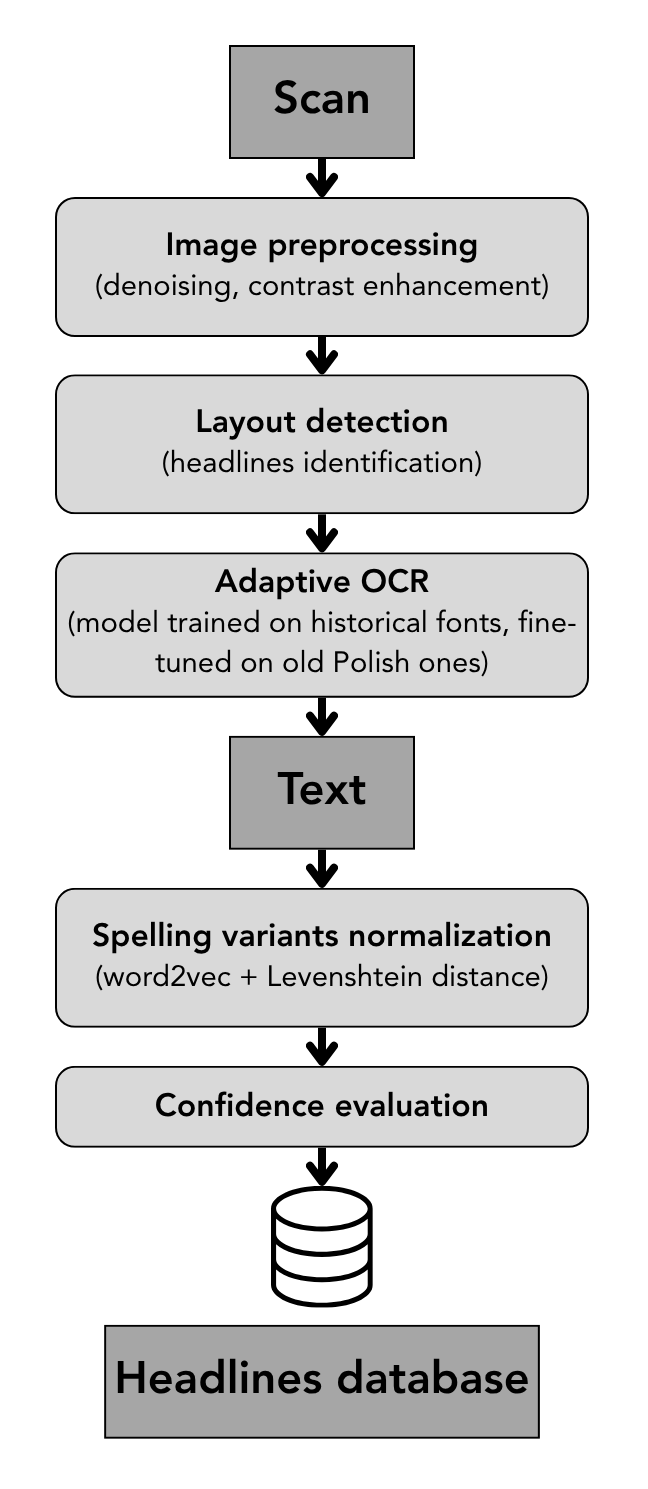
\includegraphics[width=0.45\columnwidth]{data/OCR_pipeline.png}
    \caption{Proposed pipeline for historical headline extraction and normalization.}
    \label{fig:ocr_pipeline}
\end{figure}

Headline detection is evaluated by precision and recall, OCR by character and word error rate (CER, WER). Following \newcite{koynov2025opportunities}, normalization is assessed by relative error reduction, the share of characters and words changed, and the ratio of changes to errors.

\textbf{Annotation:} A short codebook defines the four devices with Polish examples and is tested on a pilot sample. Each headline is labelled by three annotators from the cohort. Each batch also has an anchor set labelled by all annotators (to measure agreement) and gold items with fixed labels (to check codebook use). Agreement is reported per device and per period as Krippendorff's $\alpha$. The final label is the majority vote; unclear cases are decided by our team.

We compare device frequencies across periods with bootstrap confidence intervals (resampling issues). Classifiers (TF-IDF with logistic regression, fine-tuned HerBERT \cite{mroczkowski2021herbert}) are trained on contemporary headlines and evaluated per period with macro F1. We use CPUs, plus a GPU for fine-tuning if available; Table~\ref{tab:project_timeline} gives the plan.

\begin{table}[!t]
\centering
\scriptsize
\setlength{\tabcolsep}{3pt}
\begin{tabular}{@{}p{0.8cm} p{4.1cm} p{2.35cm}@{}}
\hline
\textbf{Term} & \textbf{Activities and owners} & \textbf{Risk: mitigation} \\
\hline
05.11--11.11 & Prototypes: data collection (Janek), OCR (Zofia), headline detection (Ania), annotation codebook (Gabriela) & Poor scans: use other archives \\
12.11--18.11 & Integrate and test the pipeline on a small sample; proof of concept (all) & Unclear criteria: pilot sample \\
19.11--25.11 & Exploratory data analysis, documentation, resource measurements: data and OCR (Janek, Zofia), region detection and statistics (Ania), annotation process (Gabriela) & Collection delays: prioritise balanced samples \\
26.11--02.12 & Phase 2 report, source code and rebuttals (all) & Limited compute: simpler baselines \\
03.12--09.12 & Scale collection and sampling (Janek), OCR (Zofia), headline detection (Ania), annotation batches (Gabriela) & Unusable data: other sources \\
10.12--16.12 & Annotation and disagreements (Gabriela), OCR quality (Zofia), region analysis (Ania), classifier baselines (Janek) & Annotation delays: cover all periods first \\
17.12--23.12 & Finish annotation (Gabriela), compare device frequencies (Ania), OCR error analysis (Zofia), train and test classifiers (Janek) & Incomplete labels: smaller sample \\
24.12--02.01 & Holiday buffer, outstanding tasks (all) & Reserved for delays \\
03.01--09.01 & Temporal transfer and calibration (Janek), statistical analysis (Ania), OCR errors (Zofia), annotation quality and report coordination (Gabriela) & Delays: core metrics first \\
10.01--13.01 & Final report, presentation and video (all) & Time for final revisions \\
\hline
\end{tabular}
\caption{Week-by-week plan with owners, and risks with mitigation.}
\label{tab:project_timeline}
\end{table}

\section{Administrative Declarations}

\subsection{Contribution Table}
\begin{table}[H]
\centering
\small
\begin{tabular}{@{}p{2.1cm} p{4.1cm} p{0.7cm}@{}}
\toprule
\textbf{Team Member} & \textbf{Tasks Done} & \textbf{Hours} \\ \midrule
Gabriela Majstrak &Literature review (Polish press corpora), Datasets Status (Table 2 and text), Data Statement, annotation design in Methodology & 12\\
Jan Opala & Literature review (OCR and post-OCR correction), pipeline proposal & 8 \\
Anna Ostrowska & Work plan, reading list, section 2 (beginning), 2.1 (+4 first works in Table 1); abstract; introduction, 5.2 & 11 \\
Zofia Sasimowska & Clickbait and Temporal Transfer literature review, 2.3, statistical analysis and classification methodology (4.1), week-by-week plan (Table 3) & 9.5 \\
\bottomrule
\end{tabular}
\end{table}
\subsection{Declaration of LLM Use}
We declare the use of Large Language Models Claude Opus 5.5 for the following tasks during the preparation of this report: 

1. Literature suggestions: 4 different fields/topics we should research on, and a few papers per topic. Each cited paper was read by us.

2. Autocorrection: the spellchecker built into Overleaf was used for language corrections.

3. Drafting: parts of the document were drafted with Claude based on our notes and the papers; we checked and edited them.

4. Shortening: Claude was used to condense the text and tables to fit the page limit; we checked that no content or results were changed.

\bibliographystyle{acl}
\bibliography{refs}

\end{document}